\section*{3.18}

Assume there are $p$ processors.

\begin{enumerate}
    \item[(1)] Divide array to $p$ subarrays:
        \begin{itemize}
            \item Let $r = n \mod p$
            \item First $r$ subarrays have $\left\lceil n/p \right\rceil$ elements
            \item The rest $p - r$ subarrays have $\left\lfloor n/p\right\rfloor$  elements
        \end{itemize}
    \item[(2)] Each processor $i$ scans its subarray, record the larget element $m_i$ and the second largest element $m'_i$.
    \item[(3)] Agglomerate $m_i$ and $m'_i$ from all processors to processor 0, then we get a array of $2p$ elements.
    \item[(4)] Scan the new array to get the second largest element.
\end{enumerate}

\section*{4.8}

The source code is presented as \href{run:./4_8.cpp}{4\_8.cpp}.

We first split $N$ into $p$ intervals, each processor count primes in its interval. 

\begin{lstlisting}[language=C++]
    int start = rank * (1000000 / size) + 1;
    int end = (rank + 1) * (1000000 / size) + 1;
    
    if (rank == size - 1) {
        end = 1000000;
    }

    for (int i = start; i < end; i += 2) {
        if (isPrime(i)) {
            if (isPrime(i + 2)) count++;
            else i += 2;
        }
    }
\end{lstlisting}

Then we use MPI\_Reduce to sum up the number of primes in each interval.

\begin{lstlisting}[language=C++]
    int total_count;
    MPI_Reduce(&count, &total_count, 1, MPI_INT, MPI_SUM, 0, MPI_COMM_WORLD);
    
    if (rank == 0) {
        printf("Total count: %d\n", total_count);
    }
\end{lstlisting}


The snapshot of the output is shown in Figure \ref{fig:4_8}.

\begin{figure}[H]
    \centering
    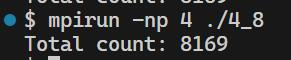
\includegraphics[width=0.3\textwidth]{fig-4.8.jpg}
    \caption{Snapshot of the output of 4.8}
    \label{fig:4_8}
\end{figure}

\section*{5.7}

The original source code is presented as \href{run:./5_7.cpp}{5\_7.cpp}, and the modified source code is presented as \href{run:./5_7_opt.cpp}{5\_7\_opt.cpp}.

Firstly, every processor will find all the prime numbers between $3$ and $\sqrt N$.

\begin{lstlisting}[language=C++]
    sqrt_n = sqrt(n);
    size = sqrt_n - 1;
    marked = new char[size / 2];
    prime = 3;
    do
    {
        first = prime * prime - 3;

        for (i = first; i < size; i += prime*2)
            marked[i/2] = 1;

        while (marked[++index]);
        prime = index *2 + 3;

    } while (prime * prime <= sqrt_n);
\end{lstlisting}

Then those primes are used to mark the table. Moreover, to reduce memory comsumption, we only store odd numbers in the table. That is, when we want to mark $x$, we actually mark $\lfloor x/2 \rfloor $.

\begin{lstlisting}[language=C++]
    while ((prime = base_primes[j]) != -1)
    {
        if (prime * prime > low_value)
        {
            first = prime * prime - low_value;
        }
        else 
        {
            if (!(low_value % prime))
                first = 0;
            else 
                first = prime - (low_value % prime);
            if ((low_value + first) % 2 == 0) first += prime;
        }
        for (i = first; i < size; i += prime*2){
            marked[i/2] = 1;
        }
        j++;
    }
\end{lstlisting}

The snapshot of the output is shown in Figure \ref{fig:5_7}.

\begin{figure}[H]
    \centering
    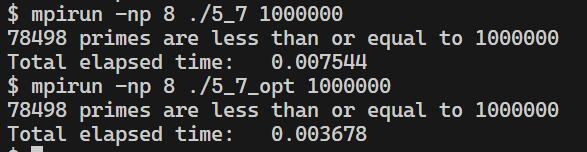
\includegraphics[width=0.6\textwidth]{fig-5.7.jpg}
    \caption{Snapshot of the output of 5.7}
    \label{fig:5_7}
\end{figure}

After optimization, the time consumption is reduced by about $50\%$.

\section*{6.9}

The source code is presented as \href{run:./6_9.cpp}{6\_9.cpp}.

Instead of using `MPT\_Reduce', we will use MPI\_Recv and MPI\_Send to implement the reduce function. All processors will send their data to the root processor, and the root processor will sum up all the data.

\begin{lstlisting}[language=C++]
    void reduce(const int *sendbuf, int *recvbuf, int count, int root) {
        int rank, size;
        int *tempbuf = new int[count];
        MPI_Comm_rank(MPI_COMM_WORLD, &rank);
        MPI_Comm_size(MPI_COMM_WORLD, &size);
        if(rank == root) {
            for (int i = 0; i < count; i++) {
                recvbuf[i] = 0;
            }
            for(int i = 0; i < size; i++) {
                if(i != root) {
                    MPI_Recv(tempbuf, count, MPI_INT, i, 
                        0, MPI_COMM_WORLD, MPI_STATUS_IGNORE);
                    for (int j = 0; j < count; j++) {
                        recvbuf[j] += tempbuf[j];
                    }
                } else {
                    for (int j = 0; j < count; j++) {
                        recvbuf[j] += sendbuf[j];
                    }
                }
            }
        } else {
            MPI_Send(sendbuf, count, MPI_INT, root, 0, MPI_COMM_WORLD);
        }
        delete[] tempbuf;
    }
\end{lstlisting}

The snapshot of the output is shown in Figure \ref{fig:6_9}.

\begin{figure}[H]
    \centering
    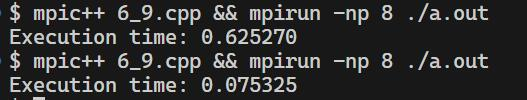
\includegraphics[width=0.6\textwidth]{fig-6.9.jpg}
    \caption{Snapshot of the output of 6.9}
    \label{fig:6_9}
\end{figure}

`MPT\_Reduce' is used in the first run, and my own implementation is used in the second run. My implementation is faster than `MPT\_Reduce', I guess it is because `MPT\_Reduce' is implemented in a more general way, and my implementation is more specific.

\section*{7.5}

With Amdahl's Law
$$
10 = \frac{1}{(1 - 0.94) + \frac{0.94}{N}}
$$
$$
N=23.5
$$

So at least $24$ processors are needed to achieve a speedup of $10$.

\section*{7.8}

The fraction of time spent in the parallel computation performing inherently sequential operations:
$$
s = \frac{9}{242} = 0.037
$$
Number of processors $p$ is $16$.
$$
\varPsi = p + s(1 - p) = 15.442
$$

So the scaled speedup is $15.442$.